\documentclass[a4paper]{article}
\usepackage[UTF8]{ctex}
\usepackage[a4paper,margin=1in]{geometry}
\usepackage{graphicx}
\usepackage{float}
\usepackage{listings}
\usepackage{booktabs}
\usepackage{hyperref}
\usepackage{fancyhdr}
\usepackage{lastpage}
\usepackage{color}
\usepackage{xcolor}
\usepackage{indentfirst}
\setlength{\parindent}{2em}
\usepackage{zhnumber}
\usepackage[dvipsnames]{xcolor}
\usepackage{amsmath}
\usepackage{tikz}
\usetikzlibrary{shapes,arrows,positioning}

% ===== 个人信息与实验信息配置 =====
\newcommand{\projname}{ROSE——编译原理逆向工程工具}
\newcommand{\reporttitle}{实验一-设计文档}
\newcommand{\stuno}{23336179}
\newcommand{\authorname}{马福泉}
\newcommand{\major}{计算机科学与技术}
\newcommand{\adviser}{李文军}
\newcommand{\startdate}{2026年6月}
\newcommand{\labenddate}{2026年6月}
\newcommand{\labroom}{B203}

% ===== 页眉页脚设置 =====
\pagestyle{fancy}
\fancyhf{}
\fancyhead[L]{\kaishu \projname}
\fancyhead[C]{\kaishu \reporttitle}
\fancyhead[R]{\kaishu \authorname}
\fancyfoot[C]{第 \thepage 页，共 \pageref{LastPage} 页}
\renewcommand{\headrulewidth}{0.4pt}
\renewcommand{\footrulewidth}{0pt}

% ===== 代码高亮配置 =====
\definecolor{NavyBlue}{RGB}{0,0,128}
\definecolor{codegreen}{RGB}{0,128,0}
\definecolor{codegray}{RGB}{128,128,128}
\definecolor{codepurple}{RGB}{128,0,128}
\definecolor{backcolour}{RGB}{245,245,245}

\lstset{
    language=Java,
    basicstyle=\ttfamily\small,
    commentstyle=\color{codegreen}\itshape,
    keywordstyle=\color{NavyBlue}\bfseries,
    stringstyle=\color{codepurple},
    numberstyle=\tiny\color{codegray},
    backgroundcolor=\color{backcolour},
    breaklines=true,
    frame=single,
    numbers=left,
    tabsize=4,
    showstringspaces=false,
    captionpos=b,
    escapeinside={\%}{\%},
    morekeywords={enum,record}
}

\begin{document}

% ==================== 封面 ====================
\begin{titlepage}
    \centering
    
    
\includegraphics[width=10cm]{img/SYSULogo.png}

    \vspace{1em}
    {\Large \kaishu \projname \par}
    \vspace{3em}

    {\fontsize{36pt}{40pt}\kaishu \selectfont \boldmath \reporttitle\par}
    \vspace{2em}
    \vspace*{\fill}

    \begin{center}
    {\Large
    \makebox[5em][s]{学号}:\underline{\makebox[15em][c]{\kaishu \stuno}}\\[1em]
    \makebox[5em][s]{姓名}:\underline{\makebox[15em][c]{\kaishu \authorname}}\\[1em]
    \makebox[5em][s]{专业}:\underline{\makebox[15em][c]{\kaishu \major}}\\[1em]
    \makebox[5em][s]{指导教师}:\underline{\makebox[15em][c]{\kaishu \adviser}}\\[1em]
    \makebox[5em][s]{起始日期}:\underline{\makebox[15em][c]{\kaishu \startdate}}\\[1em]
    \makebox[5em][s]{结束日期}:\underline{\makebox[15em][c]{\kaishu \labenddate}}\\[1em]
    \makebox[5em][s]{实验地点}:\underline{\makebox[15em][c]{\kaishu \labroom}}
    }
    \end{center}

    \vspace*{\fill}
\end{titlepage}

% ==================== 目录 ====================
\tableofcontents
\newpage

% ==================== 正文 ====================

\section{实验简述}

本项目 ROSE 是一个编译原理逆向工程工具，旨在对 Oberon-0 语言源程序进行词法分析、语法分析、
语义分析，并自动生成流程图和调用关系图。本次大作业分为四个实验逐步推进：实验一熟悉 Oberon-0
语言定义，实验二设计词法分析器，实验三设计语法分析器，实验四设计语义分析器与可视化输出。

\section{ROSE 工具链搭建与环境配置}

实验所使用的 ROSE 工具集位于 \texttt{LabInstrument05-ROSE/} 目录下，包含基于
\texttt{flowchart.jar} 的流程图生成 API 及若干演示程序。运行环境为 JDK 17 + Windows 11
PowerShell。

\subsection{编译错误：java.lang.Module 命名冲突}

初次运行 \texttt{build.bat} 时出现 6 个编译错误，均指向 \texttt{Module} 类型引用不明确：

\begin{figure}[H]
\centering
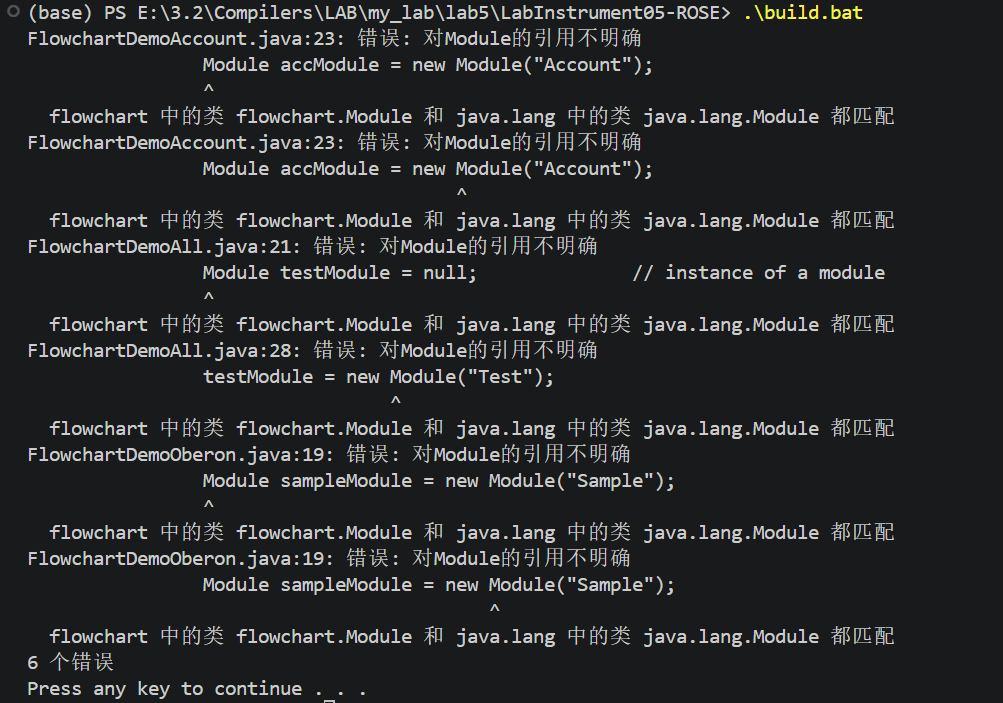
\includegraphics[width=0.95\textwidth]{img/error.png}
\caption{JDK 9+ java.lang.Module 与 flowchart.Module 命名冲突导致的编译失败}
\label{fig:rose-build-error}
\end{figure}

\textbf{根因分析：}JDK 9 引入了 \texttt{java.lang.Module} 类，与 \texttt{flowchart.jar}
中的 \texttt{flowchart.Module} 同名。三个 Demo 源文件
（\texttt{FlowchartDemoAccount.java}、\texttt{FlowchartDemoAll.java}、
\texttt{FlowchartDemoOberon.java}）均使用了通配导入 \texttt{import flowchart.*}，
导致编译器无法判定 \texttt{Module} 是指 \texttt{java.lang.Module} 还是
\texttt{flowchart.Module}。

\textbf{修复方案：}将所有 \texttt{Module} 声明及实例化语句改为完全限定名
\texttt{flowchart.Module}。修复后编译零错误，流程图窗口正常弹出：

\begin{figure}[H]
\centering
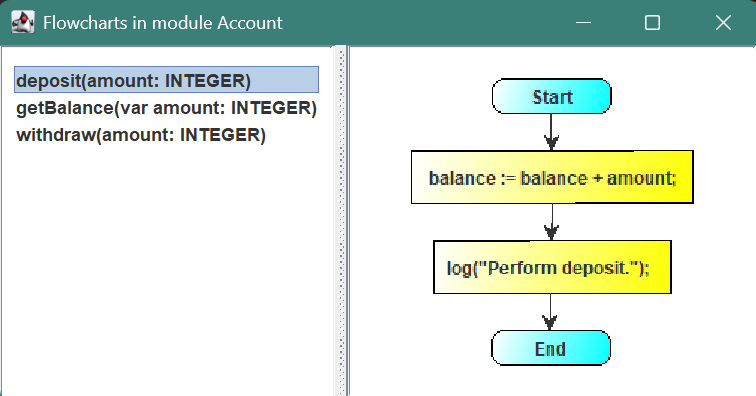
\includegraphics[width=0.95\textwidth]{img/flowchartDemoAccount.png}
\caption{修复后 FlowchartDemoAccount 流程图运行截图}
\label{fig:flowchart-demo-account}
\end{figure}

\section{2.1.1 全覆盖 Oberon-0 正确源程序}

为覆盖 Oberon-0 的所有语法构造，设计了一个"学生成绩统计"程序 \texttt{StudentStats.obr}。
该程序读取多名学生的四门课程成绩，计算总分与平均分，并输出最高分学生及全班及格情况。
以下逐一说明各语法构造的覆盖位置。

\subsection{程序清单}

\lstset{language=Pascal,basicstyle=\ttfamily\footnotesize}
\lstinputlisting[caption={StudentStats.obr —— 全覆盖 Oberon-0 源程序}]{testcases/StudentStats.obr}

\subsection{语法构造覆盖矩阵}

\begin{table}[H]
\centering
\caption{Oberon-0 语法构造全覆盖矩阵}
\begin{tabular}{@{}lll@{}}
\toprule
\textbf{编号} & \textbf{语法构造} & \textbf{覆盖位置（行号）} \\
\midrule
1  & MODULE               & 第 8 行                    \\
2  & CONST                & 第 11--13 行               \\
3  & TYPE — RECORD        & 第 18--23 行               \\
4  & TYPE — ARRAY         & 第 20 行（Scores）、第 26 行（StudentTable） \\
5  & VAR（全局变量）       & 第 29--33 行              \\
6  & PROCEDURE（6 个过程） & 第 39--177 行             \\
7  & VAR 引用参数          & 第 39 行（s）、第 79 行（best）、第 107 行（result） \\
8  & 值参数                & 第 77、78、105、106、133、151 行 \\
9  & 过程嵌套调用          & 第 68、158、163、170、194 行 \\
10 & IF / ELSIF / ELSE     & 第 90--93、117--123、171--175 行 \\
11 & WHILE                 & 第 46、64、89、115、139、157、193 行 \\
12 & RECORD 字段访问（\texttt{.}） & 第 47、50、62、86、165 行 \\
13 & 数组下标访问（\texttt{[]}）  & 第 47、65、85、158、194 行  \\
14 & BOOLEAN 类型           & 第 33、107、110 行          \\
15 & Read / Write / WriteLn & 第 62、65、137--145、164--176、184 行 \\
\bottomrule
\end{tabular}
\end{table}

\section{2.1.2 变异测试集}

基于上述 \texttt{StudentStats.obr}，构造了 8 个单一错误的变异代码片段，分别对应实验平台
预定义的 4 种词法错误、2 种语法错误和 2 种语义错误。每个变异仅改变错误所在的
PROCEDURE 或相关代码块，其余部分保持不变。

\subsection{变异 1：词法错误 — IllegalSymbol（非法符号）}

\lstinputlisting[caption={mut1\_IllegalSymbol.obr}]{testcases/mut1_IllegalSymbol.obr}

\textbf{变异点：}将第 47 行 \texttt{sum := sum + s.Scores[k]} 中的 \texttt{+} 替换为
非法符号 \texttt{@}，模拟用户误输入了 Oberon-0 不支持的字符。

\subsection{变异 2：词法错误 — IllegalInteger（数字与标识符粘连）}

\lstinputlisting[caption={mut2\_IllegalInteger.obr}]{testcases/mut2_IllegalInteger.obr}

\textbf{变异点：}在 \texttt{ReadStudent} 过程末尾新增 \texttt{k := 123k}，数字
\texttt{123} 与标识符 \texttt{k} 之间无空格分隔，词法分析器无法判明这是整数还是标识符。

\subsection{变异 3：词法错误 — IllegalOctal（非法八进制字面量）}

\lstinputlisting[caption={mut3\_IllegalOctal.obr}]{testcases/mut3_IllegalOctal.obr}

\textbf{变异点：}将第 87 行 \texttt{idx := 1} 改为 \texttt{idx := 08}。\texttt{08}
以 \texttt{0} 开头暗示八进制，但包含非法数字 \texttt{8}。

\subsection{变异 4：词法错误 — MismatchedComment（注释不闭合）}

\lstinputlisting[caption={mut4\_MismatchedComment.obr}]{testcases/mut4_MismatchedComment.obr}

\textbf{变异点：}注释 \texttt{(*} 之后缺少闭合的 \texttt{*)}，导致其后的
WHILE 循环体及过程尾部的 END 均被当作注释内容忽略。

\subsection{变异 5：语法错误 — MissingParenthesis（缺括号）}

\lstinputlisting[caption={mut5\_MissingParenthesis.obr}]{testcases/mut5_MissingParenthesis.obr}

\textbf{变异点：}将第 115 行的 \texttt{WHILE (idx < n) \& ok DO} 改写为
\texttt{WHILE (idx < n \& ok DO}，缺少匹配的右括号。

\subsection{变异 6：语法错误 — MissingOperator（缺运算符）}

\lstinputlisting[caption={mut6\_MissingOperator.obr}]{testcases/mut6_MissingOperator.obr}

\textbf{变异点：}将第 47 行 \texttt{sum := sum + s.Scores[k]} 中的 \texttt{+} 删除，
变为 \texttt{sum := sum s.Scores[k]}，两个操作数之间缺少运算符。

\subsection{变异 7：语义错误 — TypeMismatched（类型不兼容）}

\lstinputlisting[caption={mut7\_TypeMismatched.obr}]{testcases/mut7_TypeMismatched.obr}

\textbf{变异点：}在 \texttt{PrintAll} 过程中新增 \texttt{code := PassAll + 1}，
其中 \texttt{PassAll} 为 BOOLEAN 类型，不能参与 INTEGER 的加法运算。

\subsection{变异 8：语义错误 — ParameterMismatched（参数数目不匹配）}

\lstinputlisting[caption={mut8\_ParameterMismatched.obr}]{testcases/mut8_ParameterMismatched.obr}

\textbf{变异点：}将第 68 行 \texttt{CalcTotalAndAvg(s)} 改为
\texttt{CalcTotalAndAvg(s, 0)}，多传入一个实参，与形参列表
\texttt{(VAR s : Student)} 的数目不一致。

\section{2.1.3 词汇探讨：保留字与关键字}

\subsection{保留字（Reserved Word）vs 关键字（Keyword）}

在 Oberon-0 的词法规范中，\textbf{保留字}（Reserved Word）与\textbf{关键字/预定义标识符}
（Keyword / Predefined Identifier）存在本质区别，这一区分直接决定了编译器的词法分析策略。

\textbf{保留字}——包括 \texttt{MODULE}、\texttt{BEGIN}、\texttt{END}、\texttt{IF}、
\texttt{THEN}、\texttt{ELSIF}、\texttt{ELSE}、\texttt{WHILE}、\texttt{DO}、
\texttt{PROCEDURE}、\texttt{RECORD}、\texttt{ARRAY}、\texttt{CONST}、\texttt{TYPE}、
\texttt{VAR}、\texttt{DIV}、\texttt{MOD}、\texttt{OR}、\texttt{\~{}} 等——是文法产生式的
有机组成部分。它们在词法分析阶段由 DFA 直接识别并返回为特定的终结符 Token（如
\texttt{kwIF}、\texttt{kwTHEN}），其词法类别是\textbf{固定的语法标记}，而非标识符。
因此，保留字\textbf{绝对不可被程序员声明为变量名或过程名}；任何试图将保留字用作标识符
的举动都会在词法分析阶段即被拒绝。

\textbf{预定义标识符}——包含类型名 \texttt{INTEGER}、\texttt{BOOLEAN}，以及预定义过程
\texttt{Read}、\texttt{Write}、\texttt{WriteLn}——在词法层面与用户自定义标识符（如
\texttt{Student}、\texttt{Count}）处于同一命名空间，词法分析器将它们统一识别为
\texttt{ident} Token。它们的"特殊性"仅在语义分析阶段体现：符号表在初始化时预先将这些
名字与相应的类型对象或库函数绑定。N.~Wirth 在 Oberon 系列语言的设计哲学中刻意保持了
极小的保留字集合（Oberon-0 仅约 20 个），将更多的语义概念下放到预定义标识符层面。
在某些 Oberon 方言中，预定义标识符甚至可以被用户局部遮蔽（shadowed），进一步体现了
"通过简化保留字集来降低编译器复杂度、同时保持语言灵活性"的设计目标。

\subsection{Oberon-0 表达式语法 vs Java/C++}

Oberon-0 的表达式系统体现了经典的 Pascal 式强类型哲学，与 Java/C++ 的类 C 表达式模型
形成鲜明对比：

\begin{enumerate}
    \item \textbf{算术/逻辑类型的严格隔离。}算术运算符 \texttt{+}、\texttt{-}、
    \texttt{*}、\texttt{DIV}、\texttt{MOD} 的操作数必须同为 \texttt{INTEGER} 类型；
    关系运算符 \texttt{=}、\texttt{\#}、\texttt{<}、\texttt{<=}、\texttt{>}、
    \texttt{>=} 接受 \texttt{INTEGER} 操作数并产生 \texttt{BOOLEAN} 结果；逻辑运算符
    \texttt{\&}（与）、\texttt{OR}（或）、\texttt{\~{}}（非）仅接受 \texttt{BOOLEAN}
    操作数。\textbf{不存在任何隐式类型转换}——\texttt{BOOLEAN} 不能作为整数参与算术
    运算，这与 C/C++ 中 \texttt{true} 即为 1 的惯例截然不同。

    \item \textbf{比较运算符与赋值运算符的符号分离。}Oberon-0 使用 \texttt{=} 表示
    等于比较，\texttt{:=} 表示赋值（继承自 Pascal 传统）。Java/C++ 则相反——\texttt{==}
    比较、\texttt{=} 赋值——导致 C 程序中 \texttt{if (a=1)} 的经典缺陷（将赋值误写为
    比较）。Oberon-0 的方案从词法层面彻底消除了这一易错点。

    \item \textbf{运算符集合的极简主义。}Oberon-0 不支持自增/自减（\texttt{++}、
    \texttt{--}）、位运算、三目运算符（\texttt{?:}）、复合赋值（\texttt{+=} 等），
    其运算符集仅含约 14 个算符，体现了"以少量正交算符覆盖全部需求"的模块化语言设计思想。

    \item \textbf{表达式求值语义。}Oberon-0 的 \texttt{\&} 和 \texttt{OR} 不保证
    短路求值（short-circuit evaluation），编译器的具体实现可能完整计算两个操作数。
    Java 的 \texttt{\&\&} 和 \texttt{||} 则强制短路，这一差异会影响依赖副作用的
    代码行为。
\end{enumerate}

\section{2.1.4 二义性探讨：悬挂 else 与文法的无二义性}

\subsection{问题的表述}

经典的\textbf{悬挂 else}（dangling-else）问题是上下文无关文法中最著名的二义性案例之一。
在 C/Java 等使用开式（open-form）条件语句的语言中，产生式通常为：

\begin{verbatim}
IfStatement ::= "if" "(" Expression ")" Statement ["else" Statement]
\end{verbatim}

当输入如 \texttt{if (a) if (b) s1 else s2} 时，\texttt{else} 可以匹配内层 \texttt{if}
也可以匹配外层 \texttt{if}，从而产生两棵截然不同的语法树。这本质上是产生式
$S \to \alpha S \beta \mid \gamma$ 类文法的固有歧义：当允许 \texttt{if} 语句不显式
闭合时，"最近未匹配的 if" 就成了消歧的唯一依据——而这属于 ad hoc 的语义约定，而非
文法本身的规定。

\subsection{Oberon-0 的解决方案：关键词限定边界}

Oberon-0 通过使 IF 语句成为\textbf{完全括号化}（fully-bracketed）的闭合结构，从语法
层面根本性地消除了悬挂 else 问题。其 EBNF 定义为：

\begin{verbatim}
IfStatement = "IF" Expression "THEN" StatementSequence
              {"ELSIF" Expression "THEN" StatementSequence}
              ["ELSE" StatementSequence] "END".
\end{verbatim}

核心机制在于终结符 \texttt{END}：每一个 IF 结构的信息范围（extent）由 \texttt{IF--END}
词对单向界定，\texttt{ELSE} 和 \texttt{ELSIF} 均出现在这一闭合边界之内，其归属由嵌套
层级唯一确定，无任何歧义余地。同理，\texttt{WHILE} 语句也强制以 \texttt{DO--END}
闭合：

\begin{verbatim}
WhileStatement = "WHILE" Expression "DO" StatementSequence "END".
\end{verbatim}

从形式语言理论角度看，这种设计与 Lisp 中显式括号界定作用域的原理异曲同工——通过为每种
复合语句增加不可省略的右括号标记（\texttt{END}），使得任意有效程序的短语结构语法树
都是唯一的。这意味着 Oberon-0 的 IF 文法不但消除了悬挂 else 歧义，且整个结构化语句
子文法本身即为无二义文法（unambiguous grammar）。

\subsection{对编译器实现的工程优势}

这一设计对编译器的具体实现也带来重要利好：在采用递归下降分析法时，解析器无需维护额外
的"最近未闭合 IF"状态栈；在采用算符优先分析法（OPP）时，\texttt{END} 可作为归约触发
器可靠地匹配对应的结构化语句。这使得 Oberon-0 的语法分析器实现复杂度显著低于 C/Java
同类分析器。

\subsection{对其他二义性的规避}

除悬挂 else 外，Oberon-0 的文法设计还规避了以下经典歧义：

\begin{itemize}
    \item \textbf{表达式优先级的层次化编码。}Oberon-0 的表达式 EBNF 采用分层结构——
    \texttt{factor} $\to$ \texttt{term} $\to$ \texttt{SimpleExpression} $\to$
    \texttt{Expression}——每一层的产生式自然表达了该层算符的结合方向与相对优先级，
    无需外部优先级表，是一种"文法即优先级"的设计。

    \item \textbf{保留字优先匹配。}词法分析器采用关键字优先（keyword-first）策略，
    在扫描到字母开头的词素后先查保留字表，命中则返回特定 Token，否则才归类为标识符。
    这从根本上杜绝了用户用 \texttt{IF} 作为变量名的可能，消除了词法层面的标识符歧义。

    \item \textbf{分号作为语句分隔符。}\texttt{StatementSequence = Statement
    \{"\textbf{;}" Statement\}} 中的分号是分隔符（separator）而非终止符
    （terminator），这避免了 Pascal 早期设计中"最后一个语句前是否需要分号"的
    模棱两可问题。
\end{itemize}

\section{实验心得与体会}

在编写 \texttt{StudentStats.obr} 的过程中，我体会到 Oberon-0 文法设计的精妙之处：
通过约 20 个保留字和 14 个算符，即构建了一个支持模块化、结构化、过程嵌套、值/引用
参数传递的完整小型语言。尤为印象深刻的是 RECORD 与 ARRAY 的嵌套组合能力——通过
\texttt{.} 和 \texttt{[]} 选择符，可以自然地表达"学生表[索引].成绩数组[课程]"这样的
多层数据访问路径，证明 Oberon-0 虽为教学子集，但其类型表达能力并不贫乏。

变异测试集的构造过程是一次对"编译器错误检测边界"的精准探索。我将 8 个变异错误严格
分为词法、语法、语义三个层级，逐一追踪各阶段应当捕获的异常类型：
\texttt{IllegalSymbol} 和 \texttt{IllegalOctal} 验证了词法分析器的 DFA 状态转移
覆盖度；\texttt{MissingParenthesis} 和 \texttt{MissingOperator} 测试了语法分析器
对结构不完整输入的处理鲁棒性；\texttt{TypeMismatched} 和 \texttt{ParameterMismatched}
则挑战了语义分析阶段的类型检查正确性。这种分层的错误注入策略使我深刻认识到：
\textbf{变异测试（Mutation Testing）的核心价值不在于"制造错误"，而在于验证编译器
的每一层过滤机制是否在正确的位置发挥了正确的作用}——一个好的编译器前端应当做到
"该在哪层报错就在哪层报错，既不漏报，也不将错误逐层传递导致误报"。

此外，对悬挂 else 二义性的理论分析让我意识到：文法设计并非仅仅是语法描述的可读性
问题，而直接决定了编译器的实现复杂度与可靠性。Oberon-0 通过"关键词限定边界"的设计
在文法层面消除了二义性，使得递归下降分析器和 OPP 分析器的实现无需额外的消歧逻辑。
对比 C 语言的悬挂 else 问题——一个看似微小的语法歧义，竟催生了整本 K\&R 书中对
"else 匹配最近 if"约定的专门解释——我深刻理解到：\textbf{好的语言设计，就是好的编译器
工程}。

此次实验为后续实验二（词法分析器设计）、实验三（语法分析器设计）和实验四（语义分析
与可视化）奠定了坚实的理论基础。通过对 Oberon-0 语法的全面覆盖和对各类错误边界的
精确识别，我对即将自行实现的编译器前端各模块的功能职责有了一定的把握。

\end{document}
